\documentclass{beamer}

\usepackage{graphicx}
\usepackage{amsmath}
\usepackage{amsfonts}
\usepackage{amssymb}
\usepackage{tikz}
\usepackage{animate}
\usepackage{media9}
\usepackage{adjustbox}

\usepackage{multirow}   % For multi-row cells in tables
\usepackage{booktabs}   % (Optional) For better table aesthetics
\usepackage{natbib}
\usepackage{xcolor}  % needed if you define custom colors
\usepackage[normalem]{ulem}
\usepackage{subcaption}


\usetheme{Madrid}
\definecolor{myprimary}{HTML}{9792E3}
\definecolor{mysecondary}{HTML}{DB5461}


\setbeamercolor{structure}{fg=myprimary}% affects titles, bullets, etc.
\setbeamercolor{title}{fg=white,bg=myprimary}
\setbeamercolor{subtitle}{fg=myprimary}
\setbeamercolor{frametitle}{fg=white,bg=myprimary!85}
\setbeamercolor{block title}{fg=white,bg=myprimary!75}
\setbeamercolor{block body}{bg=myprimary!10, fg=black}
\setbeamercolor{itemize item}{fg=myprimary}
\setbeamercolor{itemize subitem}{fg=myprimary}
\setbeamercolor{alerted text}{fg=red!80!black} 

% \setbeamertemplate{page number in head/foot}[totalframenumber]

\newcommand{\redify}[1]{\textcolor{myprimary}{\textbf{#1}}}
\newcommand{\highlight}[1]{\textcolor{myprimary}{#1}}
\newcommand{\highlights}[1]{\textcolor{mysecondary}{#1}}

\newcommand{\notebox}[1]{\colorbox{myprimary!30}{#1}}
\newcommand{\problembox}[1]{\colorbox{mysecondary!30}{#1}}


% \AtBeginSection[]
% {
%   \begin{frame}
%     \frametitle{Table of Contents}
%     \tableofcontents[currentsection]
%   \end{frame}
% }

\newcommand{\cmark}{\ding{51}}
\newcommand{\xmark}{\ding{55}}


\newcommand{\circled}[1]{%
  \tikz[baseline=(char.base)]\node[draw=myprimary,circle,inner sep=1pt,thick,text=myprimary](char){\textbf{#1}};%
}

\title{Shaping Laser Pulses with RL}
\author[Capuano F., Peceli D., Tiboni G.]{
    Francesco \redify{Capuano}$^{(1,2)}$, 
    Davorin \redify{Peceli}$^{(3)}$, 
    Gabriele \redify{Tiboni}$^{(4,5)}$
}

\institute[]{
    \inst{1} \adjustbox{valign=c}{
\includegraphics[height=0.5cm]{images/ens-ps.png}} ENS Paris-Saclay \quad
    \inst{2} \adjustbox{valign=c}{
\includegraphics[height=0.5cm]{images/hf.png}} Hugging Face \quad
    \inst{3} \adjustbox{valign=c}{
\includegraphics[height=0.5cm]{images/elilogo.png}} ELI Beamlines \and
    \inst{4} \adjustbox{valign=c}{
\includegraphics[height=0.5cm]{images/Wurzuburg.png}} JMU Würzburg \quad
    \inst{5} \adjustbox{valign=c}{
\includegraphics[height=0.5cm]{images/Darmstandt.png}} TU Darmstadt
}

\date{\today, RLC'25}

\titlegraphic{
    
\includegraphics[width=4cm]{images/rlc-logo.png}
}

\begin{document}

%----------------------------------
\begin{frame}
  \titlepage
\end{frame}
%----------------------------------
\begin{frame}
    \frametitle{Table of Contents}
    \tableofcontents
    \end{frame}
%---------------------------------------
\section{Ultra-short Laser Pulses}

\begin{frame}[fragile]{Ultra-short Laser Pulses}
    Ultrashort ($\leq 10^{-12}$ s) laser pulses are the \redify{shortest systematic events humans can create}. They enable a range of applications, including:
\begin{columns}[T,totalwidth=\textwidth]
    \begin{column}{0.5\textwidth}
        \circled{1} \redify{Particle acceleration}
            \begin{figure}
                \animategraphics[width=0.5\linewidth,autoplay,loop]{24}{images/light-through-matter-frames/}{0}{188}
                \caption{Light traversing through matter, exchanging energy thereby accelerating particles.}
            \end{figure}
    \end{column}
    \begin{column}{0.5\textwidth}
        \circled{2} \redify{Nuclear fusion}
        \begin{figure}
            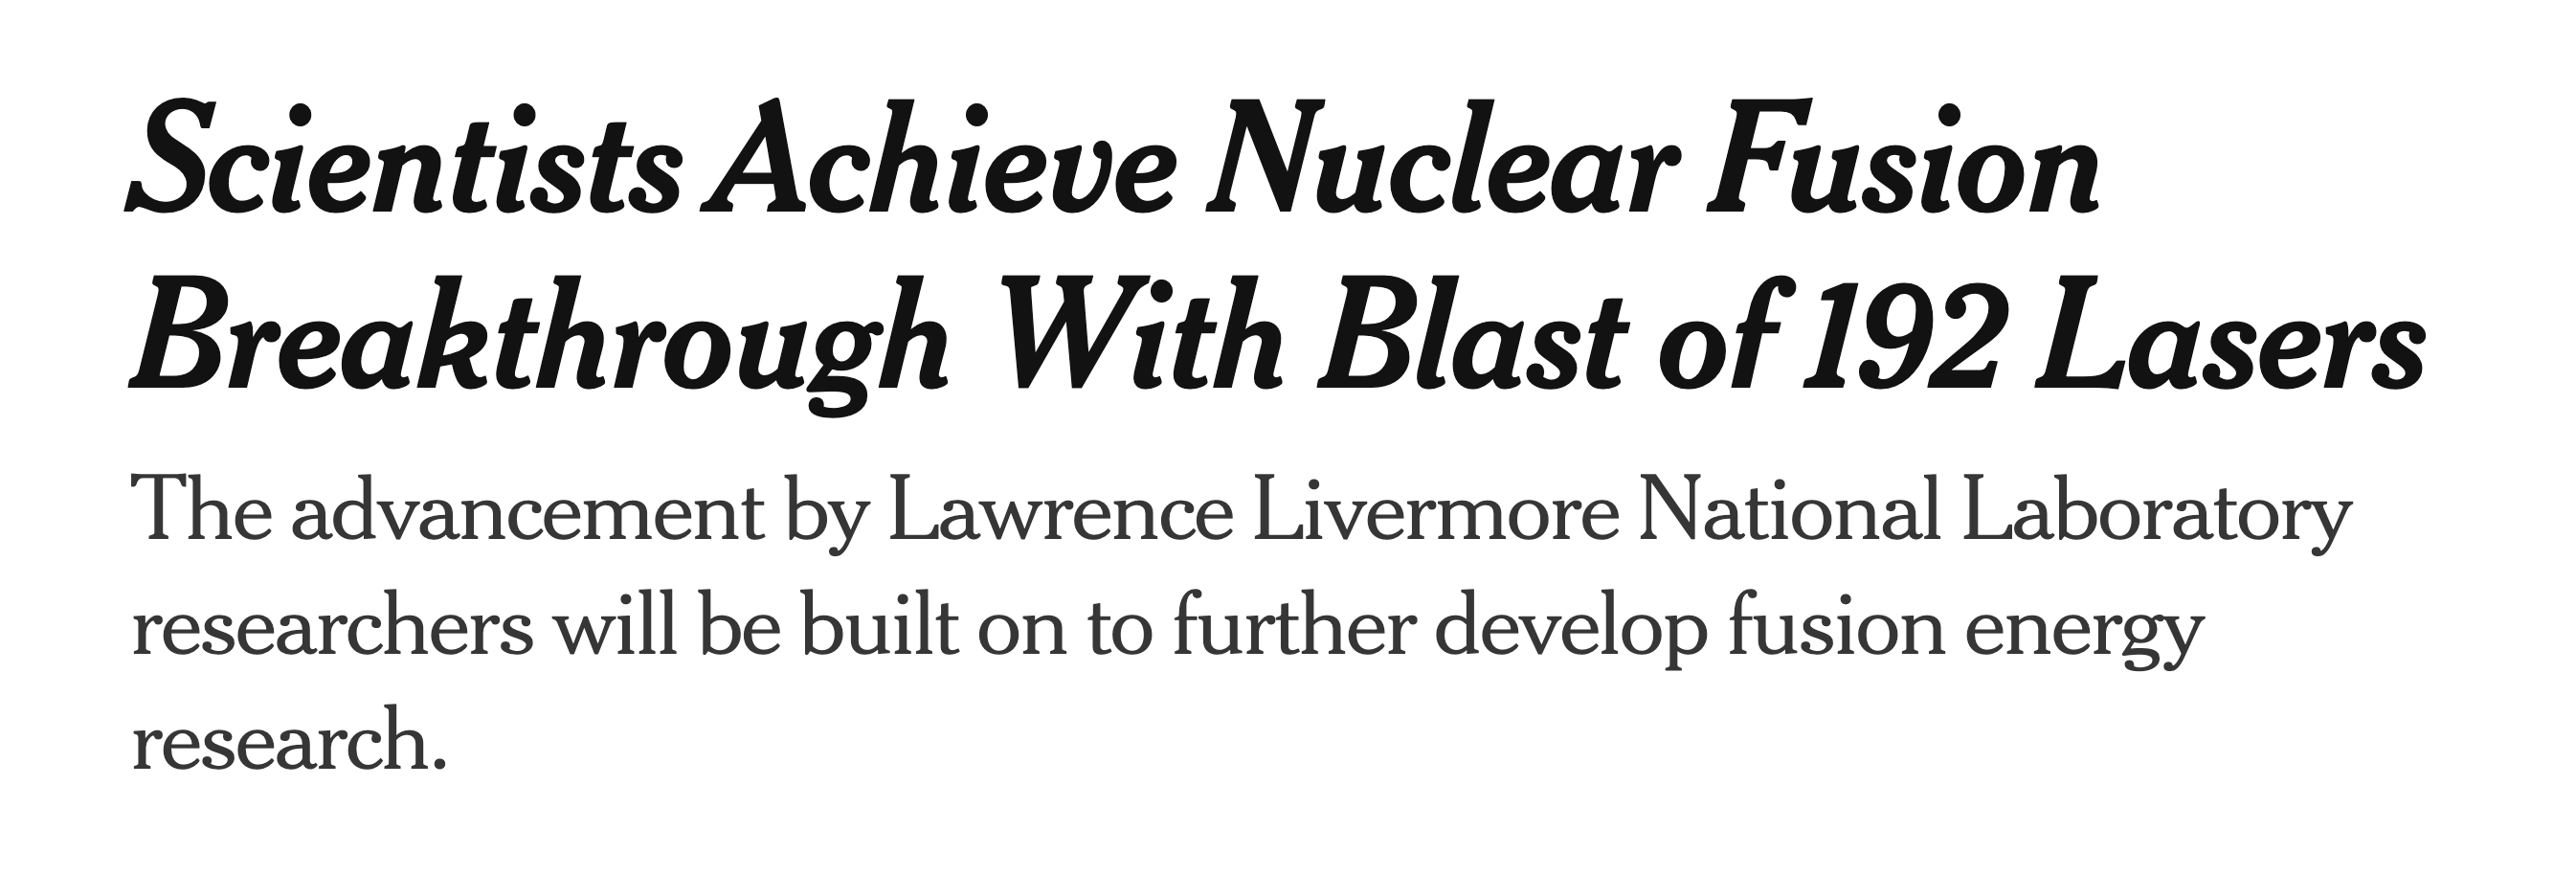
\includegraphics[width=\linewidth]{images/nuclear-nyt.png}
            \caption{NYT covering laser bursts used to achieve nuclear fusion ignition at the LLNL (USA), 2022.}
        \end{figure}
    \end{column}
\end{columns}

\end{frame}
%---------------------------------------
\begin{frame}{Maximize Intensity by Minimizing Duration}
    Laser bursts convey energy in both \highlight{time} and \highlight{space}.
    \begin{figure}
        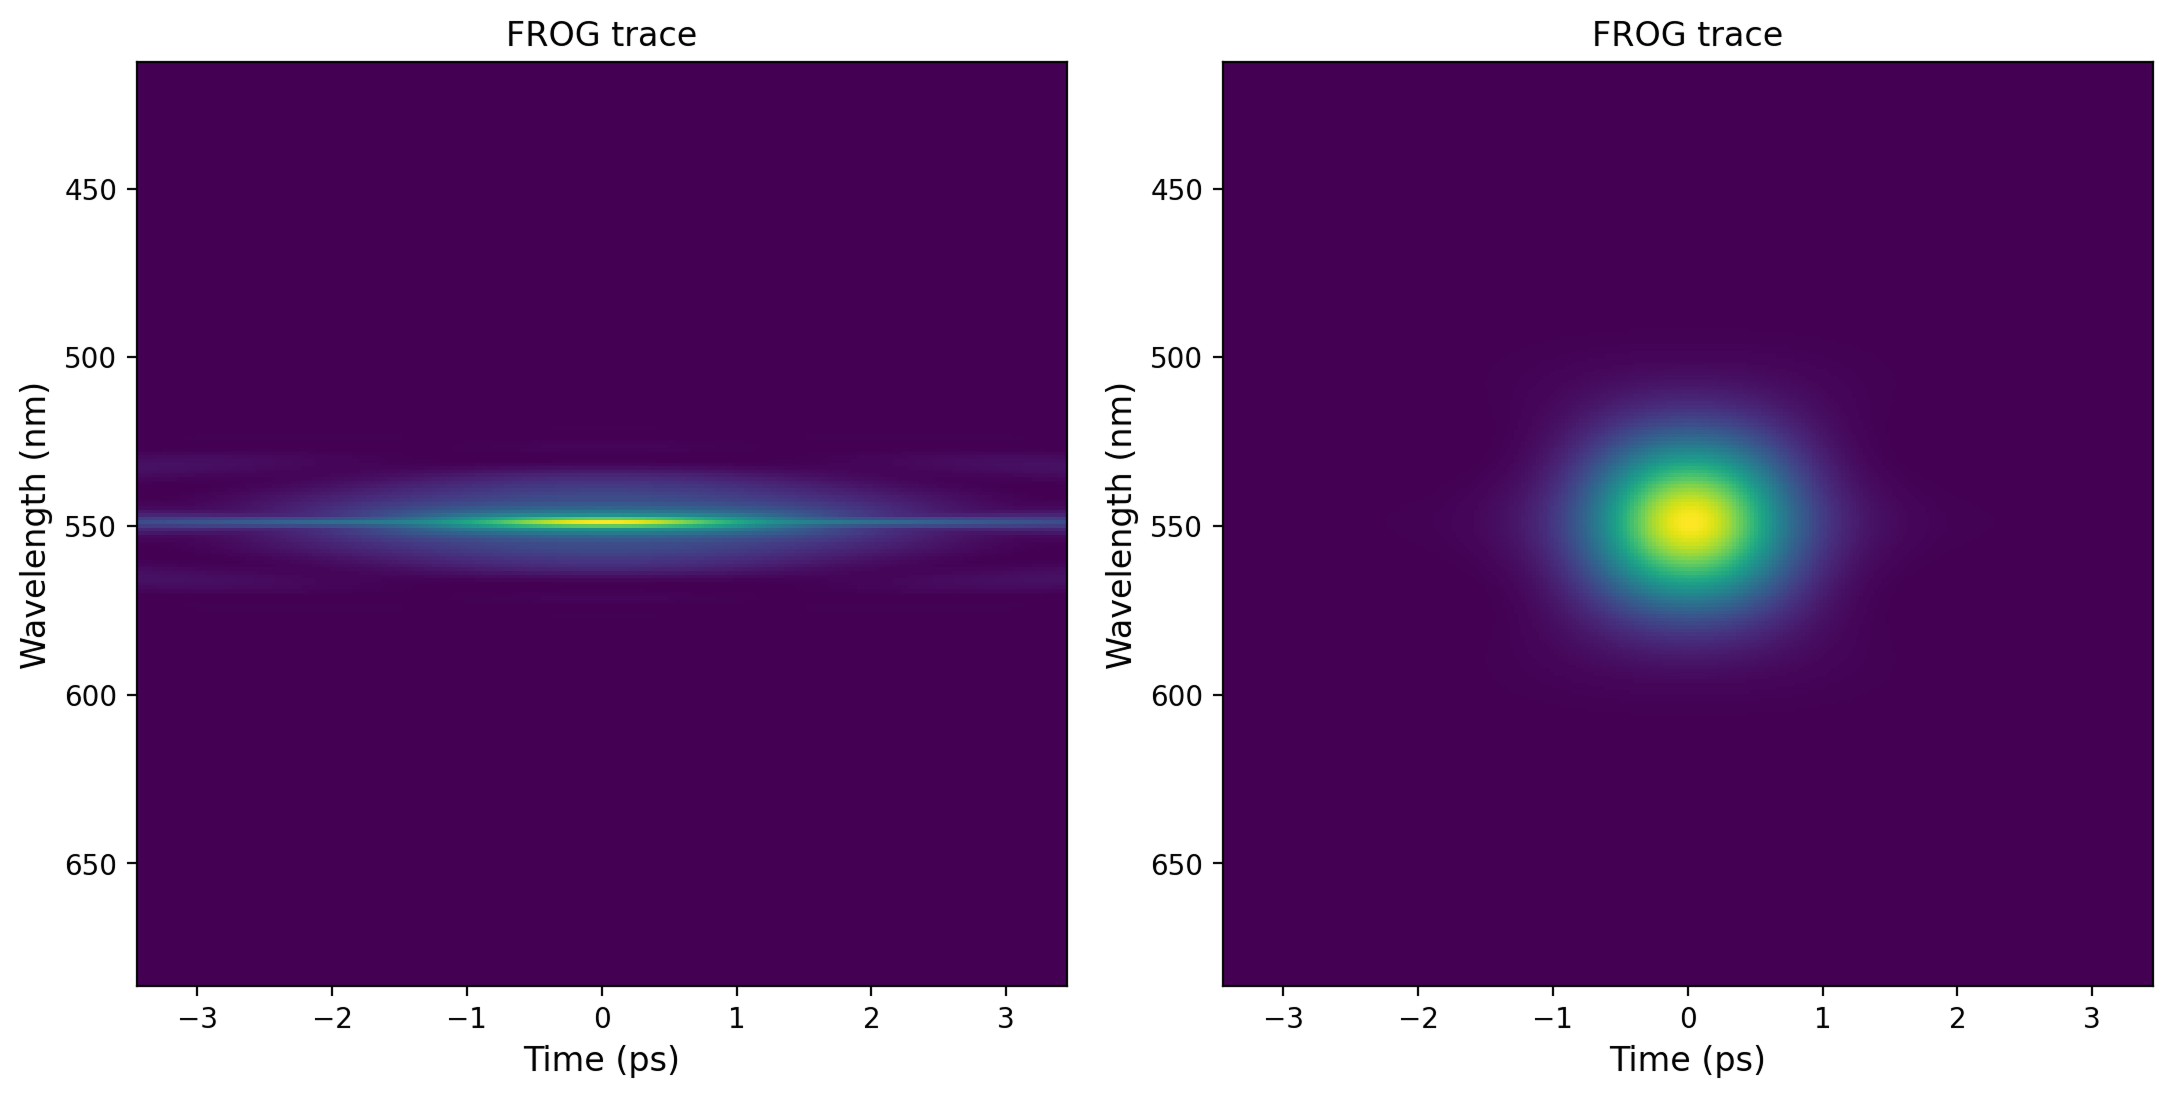
\includegraphics[width=0.4\textwidth]{images/frogs.png}
        \caption{(left) Poorly temporally-focused pulse (right) Temporally-focused pulse}
    \end{figure}
    Particle acceleration \& fusion ignition both require high-intensity bursts.
    \[
        PI_t \propto \frac{2E}{\int I_\psi(t) dt}
    \]
    \highlight{Intensity grows when:}
    \begin{itemize}
        \item Increases in the pulse energy, $E \uparrow$
        \item Decreases in pulse duration \notebox{$\int I_\psi(t) dt \downarrow$}
    \end{itemize}
\end{frame}
%---------------------------------------
\section{Shaping Laser Pulses}
\begin{frame}[fragile]{Minimizing Duration = Optimal Shaping}
    \begin{figure}
        \animategraphics[width=0.45\linewidth,autoplay,loop]{10}{images/phase-control-frames/}{0}{9}
        \caption{(left) Spectral pulse, phase in yellow (right) Resulting temporal profile.}
    \end{figure}
    Controlling the phase \redify{in the frequency domain} impacts the pulse's duration \redify{in the temporal domain}. Shaping consists of:
    \begin{itemize}
        \item \circled{1} Stretching the pulse into fundamental frequencies
        \item \circled{2} Amplifying the different frequencies (\redify{non-linear})
        \item \circled{3} Recompressing in time, aligning frequencies yielding \highlight{constructive interferences}
    \end{itemize}
\end{frame}
%---------------------------------------
\begin{frame}{Minimizing Duration = Optimal Shaping}
    \begin{figure}
        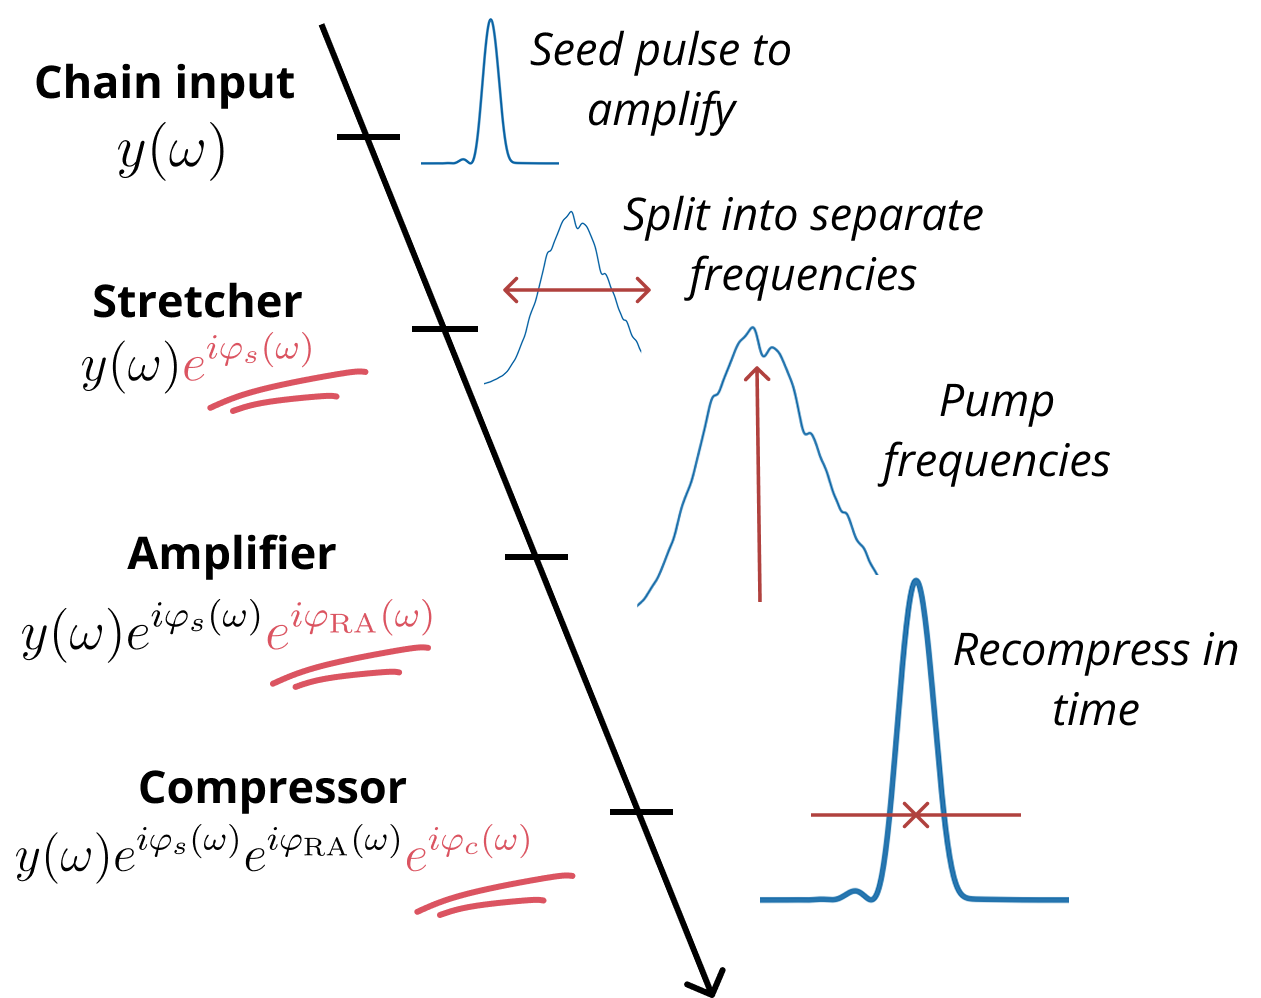
\includegraphics[width=0.45\linewidth]{images/shaping-phase.png}
    \end{figure}
    Controlling the phase \redify{in the frequency domain} impacts the pulse's duration \redify{in the temporal domain}.
        \begin{itemize}
            \item \circled{1} \notebox{Stretching the pulse into fundamental frequencies} \highlight{Can control} 
            \item \circled{2} Amplifying the different frequencies (\redify{non-linear}) \highlights{Can't control}
            \item \circled{3} Recompressing in time, aligning frequencies yielding \highlight{constructive interferences} \highlights{Can't control}
        \end{itemize}
\end{frame}
%---------------------------------------
\begin{frame}{Shaping feels like "Anon, \textit{ngmi}"}
    \uncover<+->{
    \circled{1} \redify{State reconstruction}
        \begin{itemize}
        \item Lasting pico/attoseconds, ultra-short temporal profiles \redify{cannot be directly measured}.
        \item Measuring the intensity achieved is a \redify{destructive process}.
        \end{itemize}
    }
    \uncover<+->{
    \circled{2} \redify{(Unknown-)Dynamics dependant}
    \begin{itemize}
        \item Shaping system's \redify{parameters change day by day}, and not always for fully modelled reasons.
        \item The processes of non-linear amplification and phase accumulation themselves are not fully understood
        \end{itemize}
    }
    \uncover<+->{
    \circled{3} \redify{Fragile in real-world settings}
    \begin{itemize}
        \item Real-world shapers are delicate machines needing proper care relatively to the control applied
        \item Besides being correct, \redify{controls need to be appropriate}, both in absolute and relative terms.
    \end{itemize}
    }
\end{frame}
%---------------------------------------
\section{Deep RL for Laser Pulses}
\begin{frame}{Deep RL to the rescue (1/3)}
    \begin{center}
        \circled{1} \redify{Use unstructured observations}
    \end{center}
    Bypass noisy pulse reconstructions, use raw diagnostics \redify{(images)} only. Diagnostic measurements are \redify{not destructive}.
    \begin{columns}[T,totalwidth=\textwidth]
    \begin{column}{0.7\textwidth}
        \centering
        \begin{figure}
            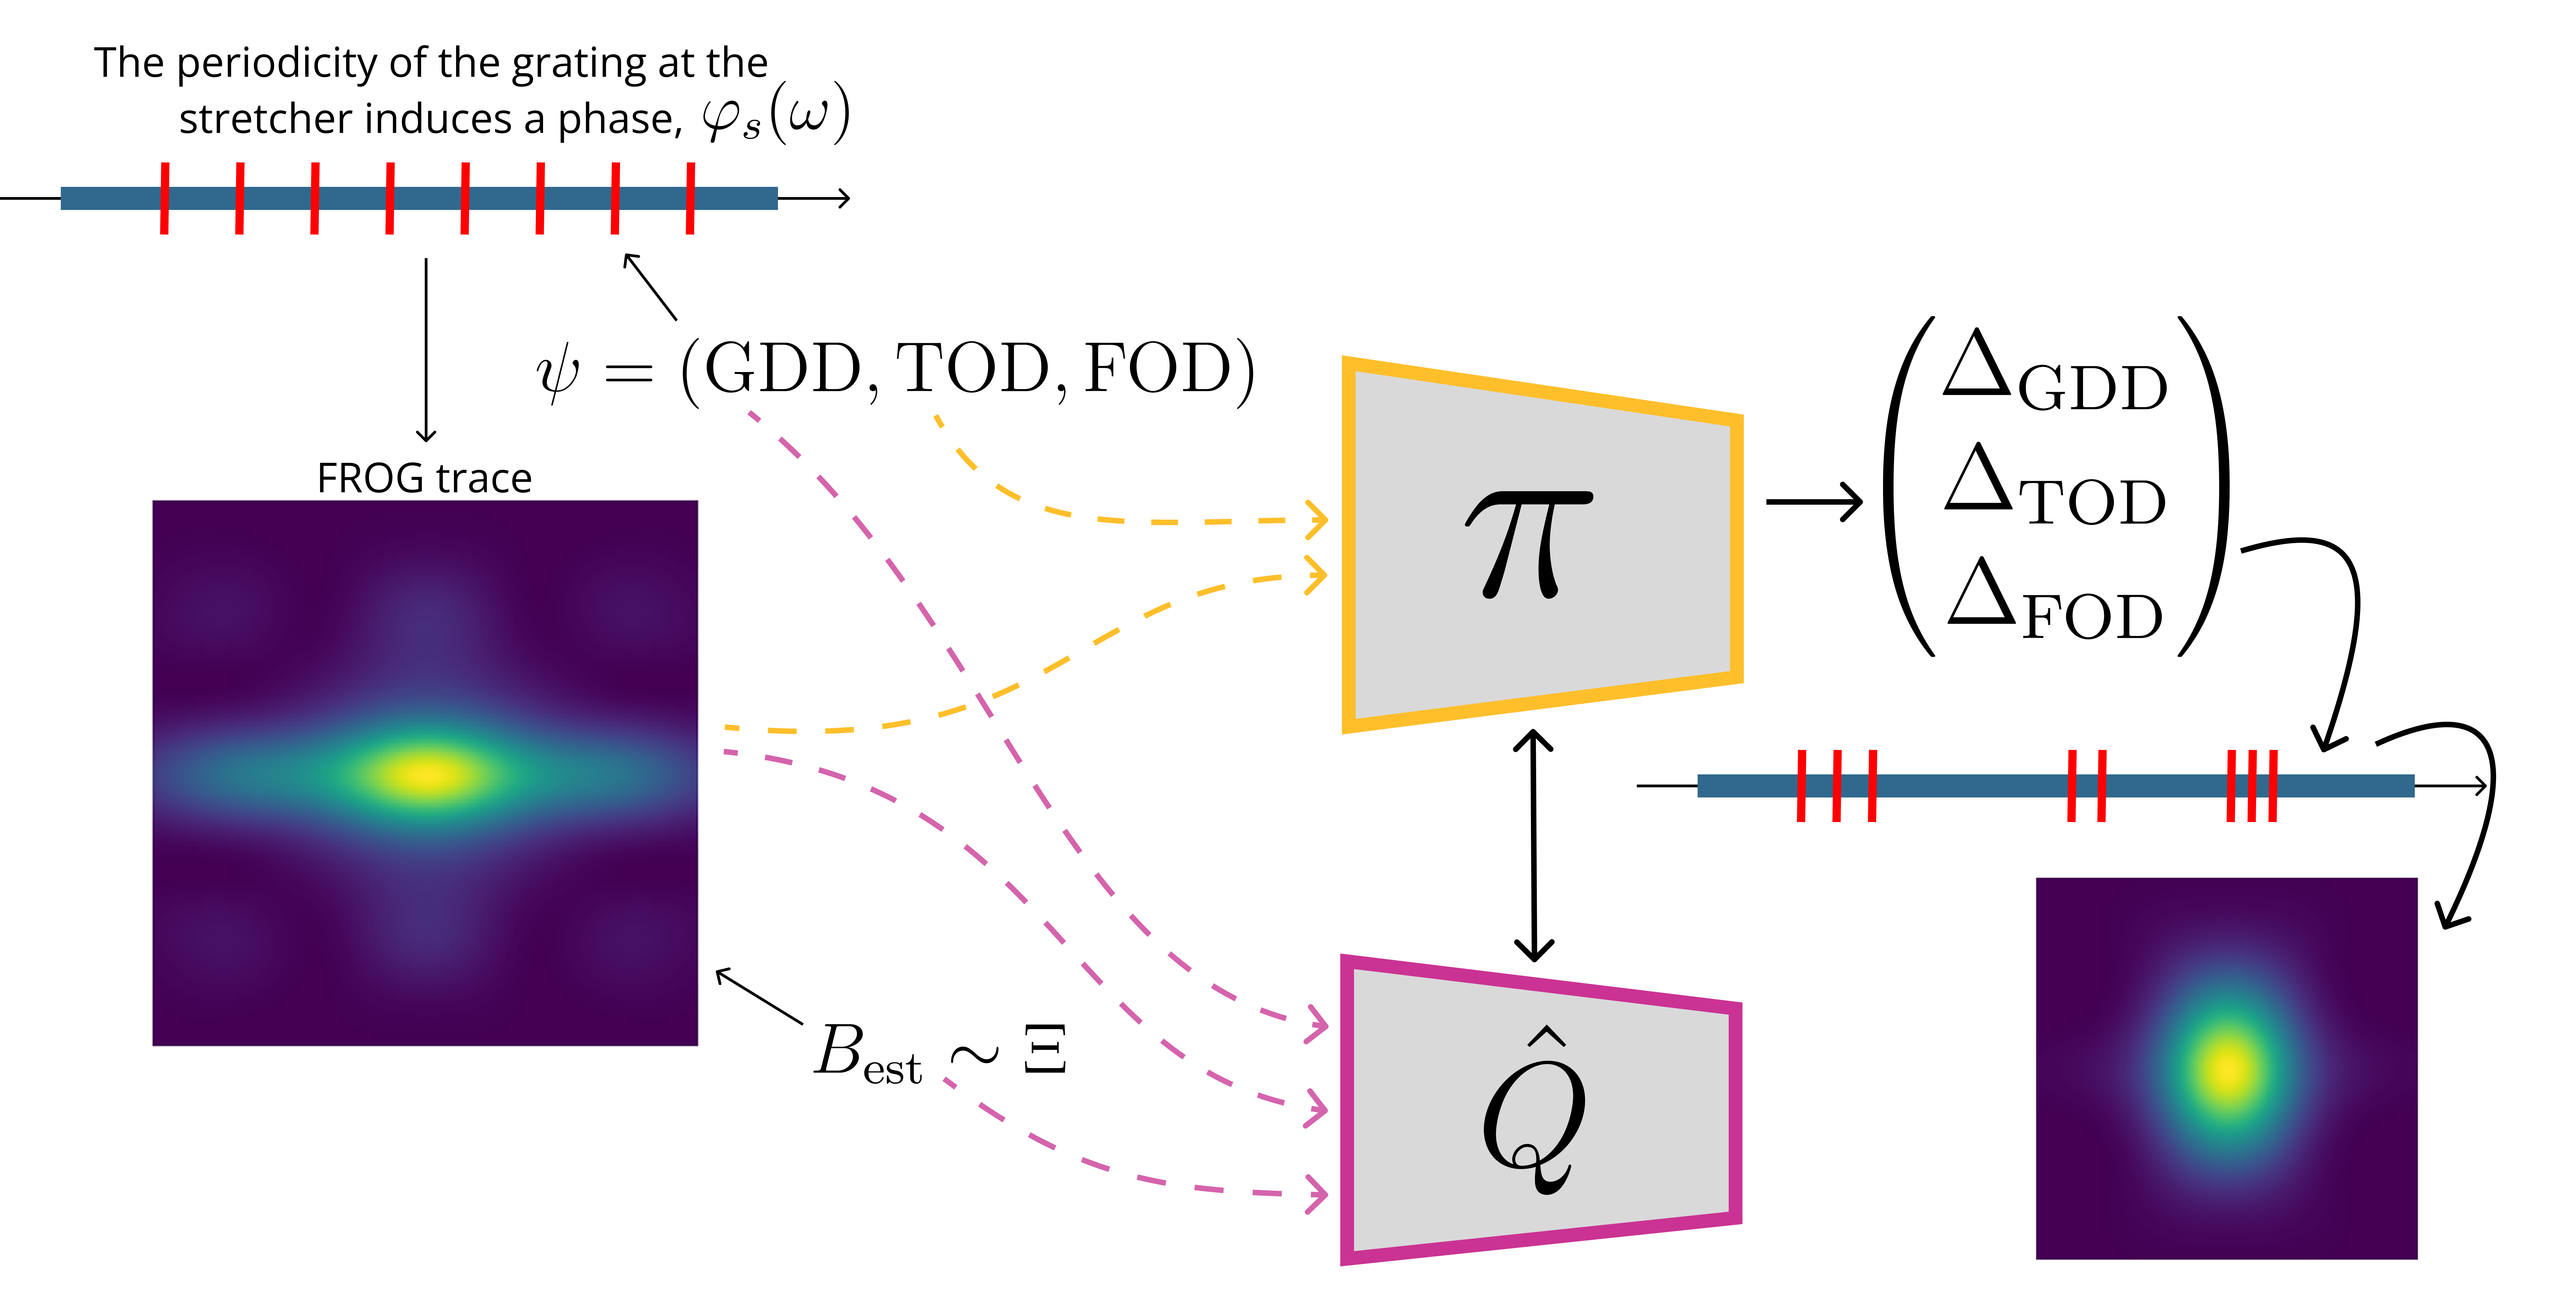
\includegraphics[width=\linewidth]{images/Figure1.png}
        \end{figure}
    \end{column}
    \begin{column}{0.3\textwidth}
        \begin{figure}
            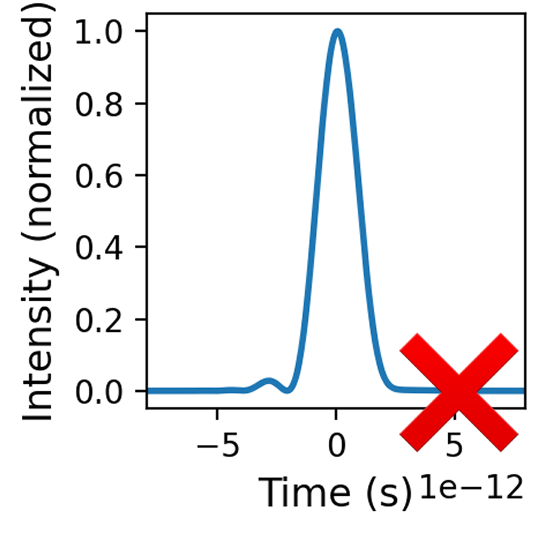
\includegraphics[width=0.6\linewidth]{images/rl-prob-1.png}
        \end{figure}
        \begin{figure}
            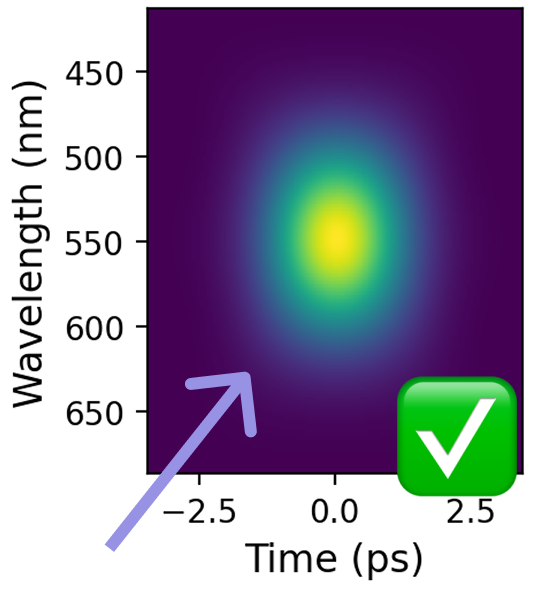
\includegraphics[width=0.6\linewidth]{images/rl-sol-1.png}
        \end{figure}
    \end{column}
\end{columns}
\end{frame}
%---------------------------------------
\begin{frame}{Deep RL to the rescue (2/3)}
    \begin{center}
        \circled{2} \redify{Induce robustness to dynamics}
    \end{center}
    \redify{Automatically adapt the randomization distribution} based on performance during training \footnote{"Domain randomization via entropy maximization", Tiboni et al., ICLR 2024}
    \begin{columns}[T,totalwidth=\textwidth]
    \begin{column}[t]{0.5\textwidth}
        \centering
        \begin{figure}
            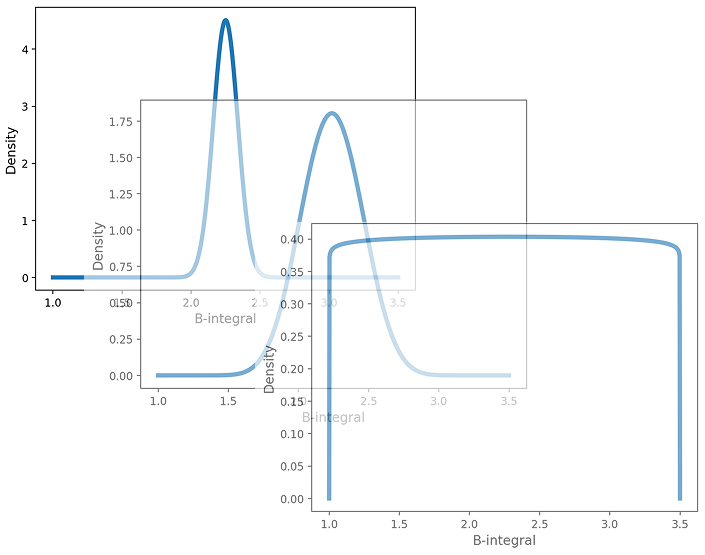
\includegraphics[width=\linewidth]{images/rl-sol-2.png}
        \end{figure}
    \end{column}
    \begin{column}[t]{0.5\textwidth}
        \begin{figure}
            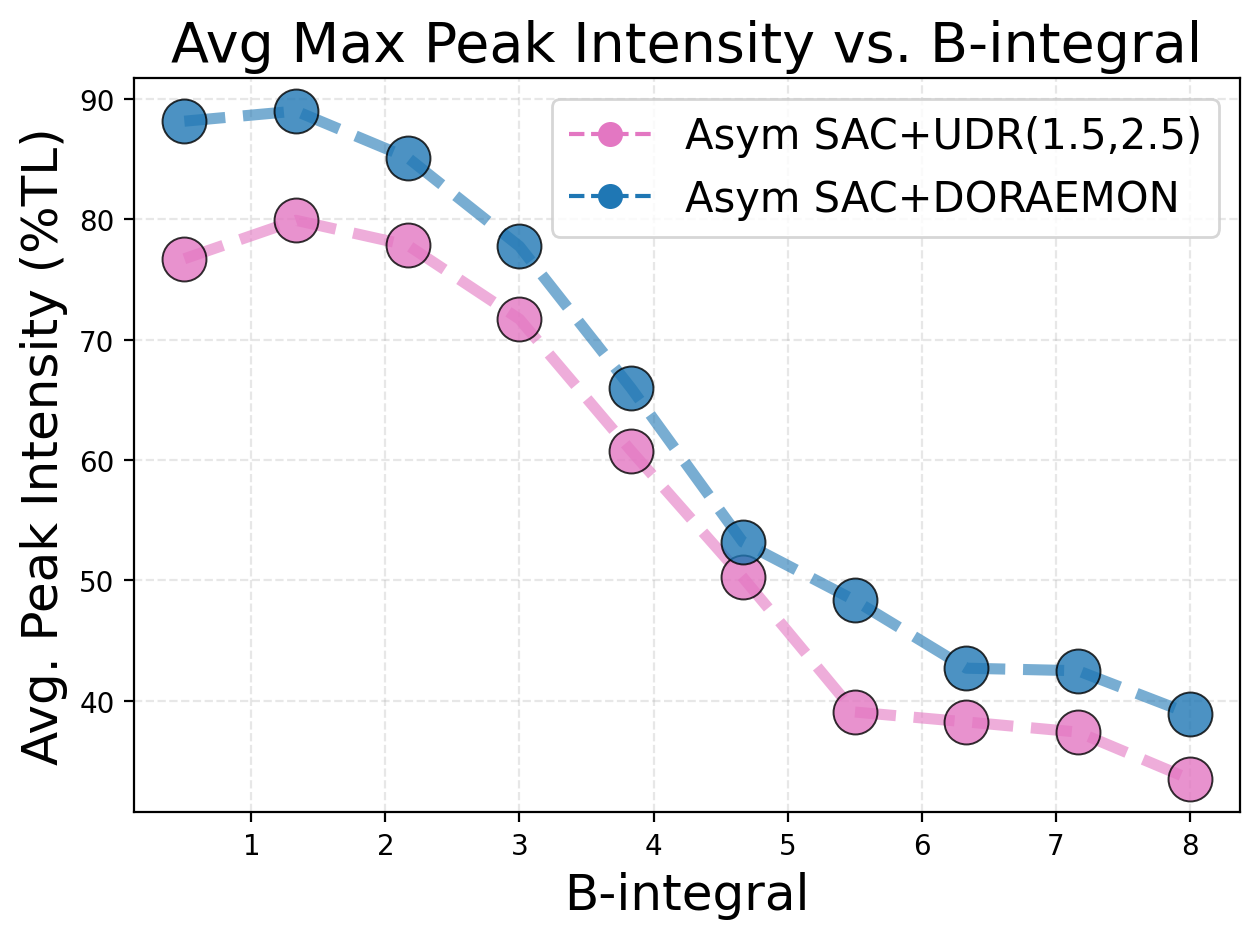
\includegraphics[width=\linewidth]{images/udr_vs_doraemon_average.png}
        \end{figure}
    \end{column}
    \end{columns}
\end{frame}
%---------------------------------------
\begin{frame}[fragile]{Deep RL to the rescue (3/3)}
    \begin{center}
    \circled{3} \redify{Train in a (coarse) simulator}
    \end{center}
    Avoid exploration on real-world systems by \redify{training in simulation}, allocating erratic behavior to in-simulation training
    \begin{columns}[T,totalwidth=\textwidth]
    \begin{column}{0.5\textwidth}
        \centering
        \begin{figure}
            \animategraphics[width=\linewidth,autoplay,loop]{24}{images/erratic-control-frames/}{0}{448}
        \end{figure}
    \end{column}
    \begin{column}{0.5\textwidth}
        \begin{figure}
            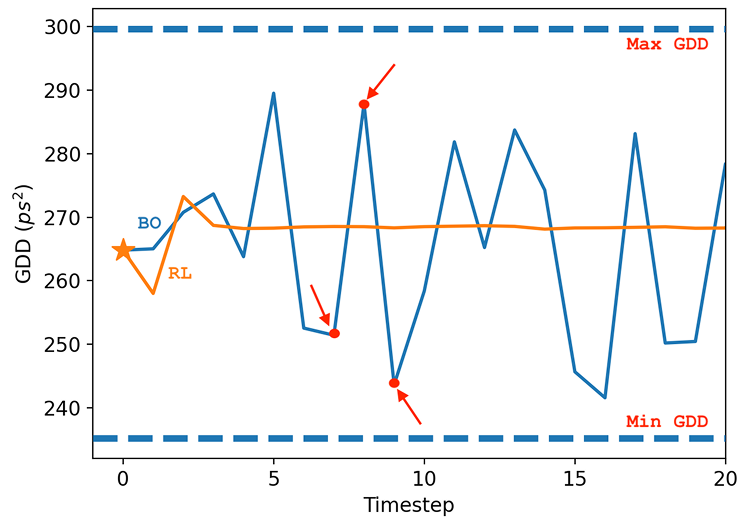
\includegraphics[width=\linewidth]{images/rl-sol-3.png}
        \end{figure}
    \end{column}
    \end{columns}
\end{frame}
%---------------------------------------
\begin{frame}[fragile]{Deep RL for pulse shaping}
    \begin{columns}
        \begin{column}{0.5\textwidth}
            \centering
            \circled{1} \redify{Asymmetric \\ Soft Actor-Critic} \\
            \notebox{Augment observations} fed to the critic network with the dynamics parameters, \( B_{\text{est.}} \).
        \end{column}
        \begin{column}{0.5\textwidth}
            \circled{2} \redify{Entropy-driven \\ Domain Randomization} \\
            \notebox{Avoid manually tuning} \( \Xi : B_{\text{est.}} \sim \Xi \), adapting it based on training signal.
        \end{column}
    \end{columns}
    \vspace{1em}
    
    We train a controller to \redify{safely tune} laser parameters for intensity maximization \redify{across dynamics} and using \redify{image observations only}.
    \begin{figure}
        \animategraphics[width=0.9linewidth,autoplay,loop]{12}{images/environment-rendering-frames/}{0}{143}
    \end{figure}
\end{frame}
%---------------------------------------
\begin{frame}{Conclusions}
We present a new method for shaping laser pulses using Deep RL, striving towards \redify{real-world usage} on the world's \redify{most powerful laser system}.
\begin{itemize}[<+->]
   \item We learn from images only, bypassing noisy state reconstruction.
   \item We train policies robust to changes in the dynamics thanks to entropy-driven DR.
   \item We train in simulation, ensuring (safe) exploration leveraging results on cross-domain transferability.
\end{itemize}

\vspace{1em}
\uncover<+->{
Environment code \notebox{\texttt{gym-laser}} \& testbed are both online and \redify{open-source}!

\centering
\begin{columns}
    \begin{column}{0.2\textwidth}
        
\includegraphics[width=\linewidth]{images/env-qr.png}
    \end{column}
    \begin{column}{0.2\textwidth}
        
\includegraphics[width=\linewidth]{images/space-qr.png}
    \end{column}
\end{columns}
}

\end{frame}
% ----------------------------------------
\begin{frame}
    Questions? \notebox{Poster 21}
    \begin{figure}
        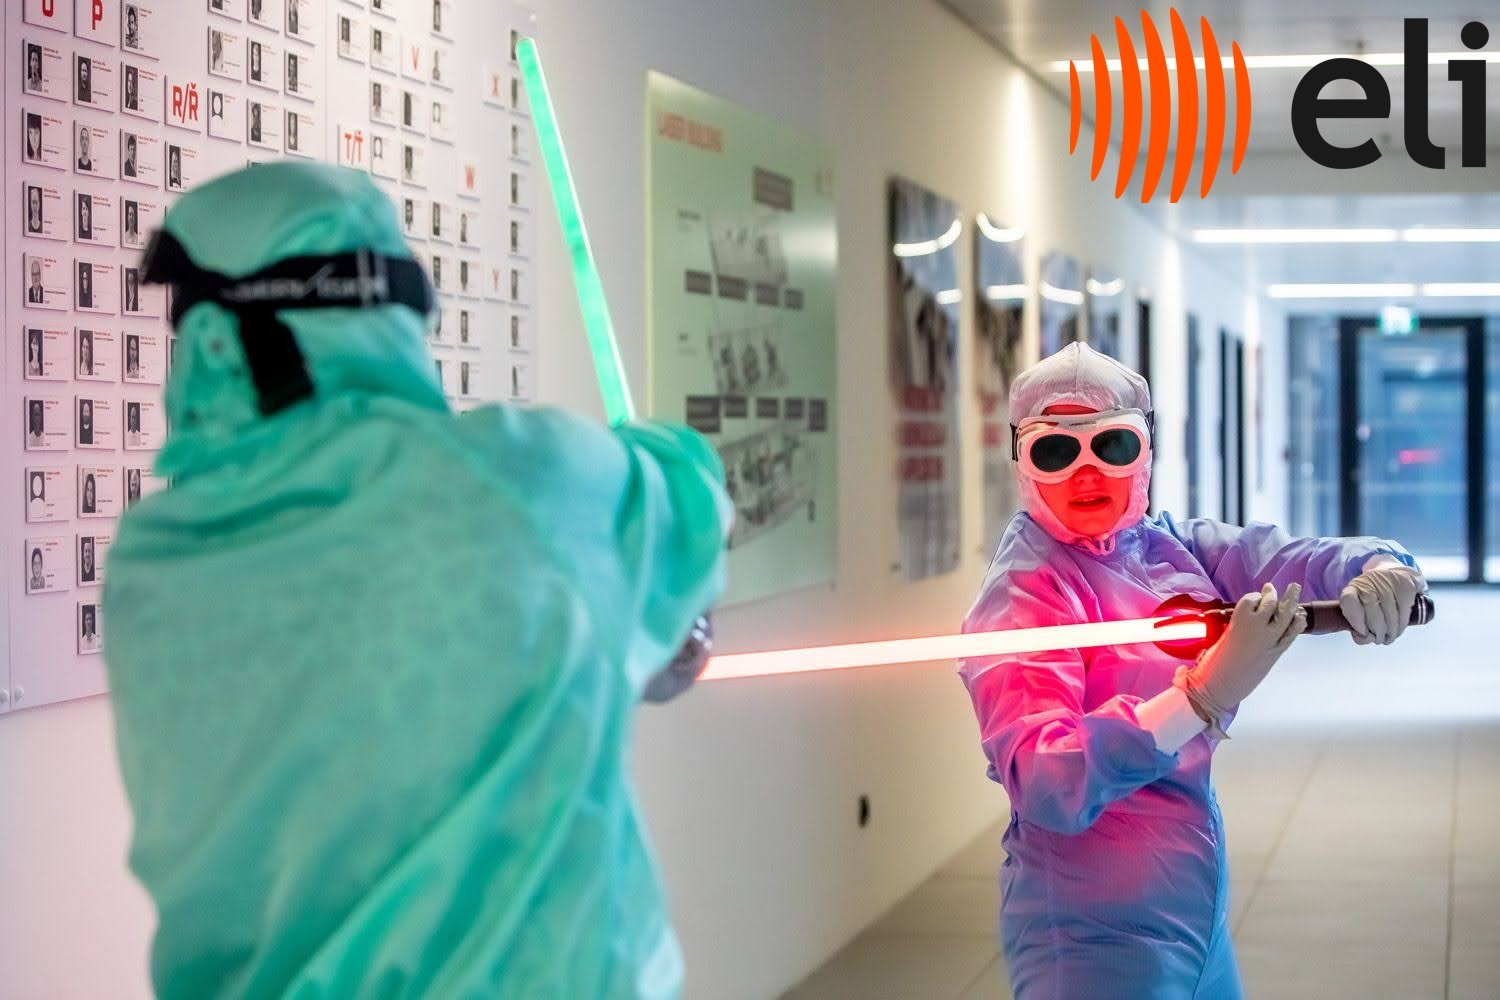
\includegraphics[width=0.6\textwidth]{images/sabers.jpg}
    \end{figure}
\end{frame}
% ----------------------------------------
\end{document}
